\section{PHƯƠNG PHÁP NGHIÊN CỨU}
	\subsection{Cơ sở Lý thuyết và Tổng quan Kiến trúc Hệ thống}
	
	\subsubsection{Khung lý thuyết về Ý định và Hành vi lái xe}
	Trong lĩnh vực xe tự hành và hệ thống hỗ trợ người lái tiên tiến (ADAS), quá trình ra quyết định của một phương tiện tham gia giao thông được mô hình hóa qua hai cấp độ: ``Ý định'' và ``Hành vi''. 
	Theo mô hình nhận thức của tài xế (Human Driver Model), "ý định" là một trạng thái tâm lý tiềm ẩn (latent state) diễn ra bên trong não bộ của người điều khiển (ví dụ: muốn vượt xe, muốn rẽ phải) trước khi các thao tác cơ học được thực thi. Trạng thái tiềm ẩn này sau đó sẽ chuyển hóa thành "hành vi" quan sát được trên không gian vật lý (như tăng tốc, đánh lái, thay đổi góc nghiêng) và cuối cùng hình thành nên quỹ đạo (trajectory) của phương tiện. Do đó, việc dự đoán "ý định" mang tính chất đi trước thời gian (proactive) và cung cấp cảnh báo sớm hơn đáng kể so với việc chỉ theo dõi "hành vi" đè vạch hay hồi quy quỹ đạo tọa độ thuần túy.
	
	\subsubsection{Đặc tính Động lực học trong Giao thông Hỗn hợp}
	Giao thông hỗn hợp tại Việt Nam đặc trưng bởi sự thống trị của xe gắn máy hai bánh (Powered Two-Wheelers - PTWs). Khác với ô tô vốn bị ràng buộc khắt khe bởi tính vật lý phi toàn hướng và thường di chuyển theo luồng tuyến tính, xe máy sở hữu đặc tính động lực học phức tạp hơn nhiều. 
	Xe máy có kích thước nhỏ, tỷ lệ công suất trên trọng lượng lớn, biên độ đánh lái rộng và đặc biệt là khả năng ``di chuyển phi làn đường''. Trong môi trường ùn tắc, người điều khiển xe máy thường xuyên thực hiện các hành vi phi tuyến tính như lách qua khe hẹp, điền vào chỗ trống, và tạt đầu ngoặt nghèo ở cự ly cực ngắn. Sự linh hoạt này khiến các mô hình dự đoán dựa trên định luật vật lý động học tiêu chuẩn (như Vận tốc không đổi - CV, hay Gia tốc không đổi - CA) hoàn toàn thất bại về mặt lý thuyết, buộc hệ thống phải chuyển sang phương pháp học máy thống kê.
	
	\subsubsection{Đề xuất Kiến trúc Lai}
	Các phương pháp truyền thống trong dự đoán chuyển động thường tách biệt bài toán thành hai giai đoạn rời rạc: phát hiện vật thể và hồi quy quỹ đạo tương lai, như đã được tổng hợp trong các khảo sát của nhóm Lefèvre \cite{Lefvre2014ASO} và nhóm Mozaffari \cite{Mozaffari2020DeepLV}. Tuy nhiên, trong môi trường giao thông hỗn hợp với mật độ cao, độ trễ tích lũy giữa các module này có thể làm giảm hiệu quả cảnh báo thời gian thực.
	
	Để khắc phục, nghiên cứu đề xuất kiến trúc End-to-End Risk Awareness. Hệ thống sử dụng Mạng nơ-ron tích chập (CNN) để trích xuất đặc trưng không gian và Mạng bộ nhớ ngắn hạn dài hạn (LSTM) để giải mã chuỗi thời gian, từ đó phân loại trực tiếp ý định tạt đầu trước khi hành vi thực sự diễn ra.
	
	Quy trình xử lý gồm 3 giai đoạn chính:
	\begin{figure}[h]
		\centering
		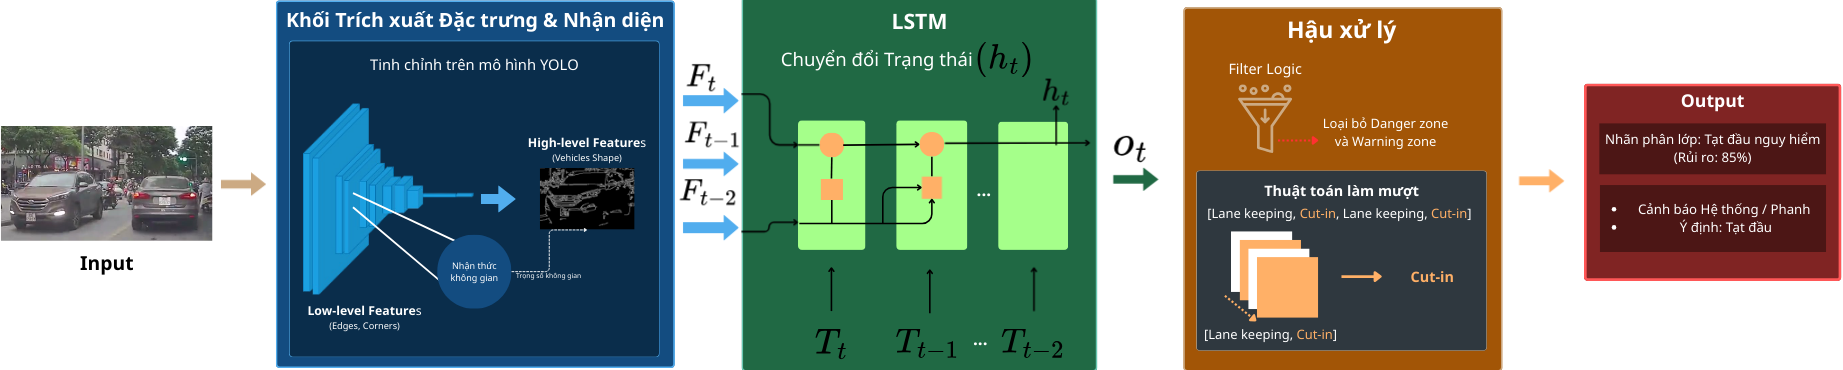
\includegraphics[width=\linewidth, height=5.5cm]{images/model_pipeline.png} 
		\caption{Sơ đồ tổng quan mô hình}
		\label{fig:model_pipeline}
	\end{figure}
	
	\begin{enumerate}
		\item Xây dựng Dữ liệu: Sử dụng quy trình bán tự động Human-in-the-loop.
		\item Mô hình Nhận thức Hành vi: Sử dụng kiến trúc YOLO tinh chỉnh.
		\item Hậu xử lý Thời gian thực: Ổn định tín hiệu cảnh báo.
	\end{enumerate}	
	
	\subsection{Phương pháp Xây dựng Dữ liệu}
	
	Để giải quyết thách thức về khối lượng dữ liệu lớn và giảm thiểu chi phí nhân lực cho việc gán nhãn thủ công, đề tài đề xuất quy trình xử lý dữ liệu hai giai đoạn theo cơ chế "Human-in-the-loop" \cite{Branson2010VisualRW}. Cách tiếp cận này tận dụng một mô hình máy học sơ khởi ($M_{assist}$) để tự động đề xuất nhãn, chuyển vai trò của con người từ "người dán nhãn" sang "người kiểm định", đảm bảo nguyên tắc AI lấy con người làm trung tâm \cite{Shneiderman2020HumanCenteredAI}.
	
	Quy trình tổng thể được mô tả tại Hình \ref{fig:data_pipeline}, bao gồm hai giai đoạn chính:
	
	\begin{figure}[h]
		\centering
		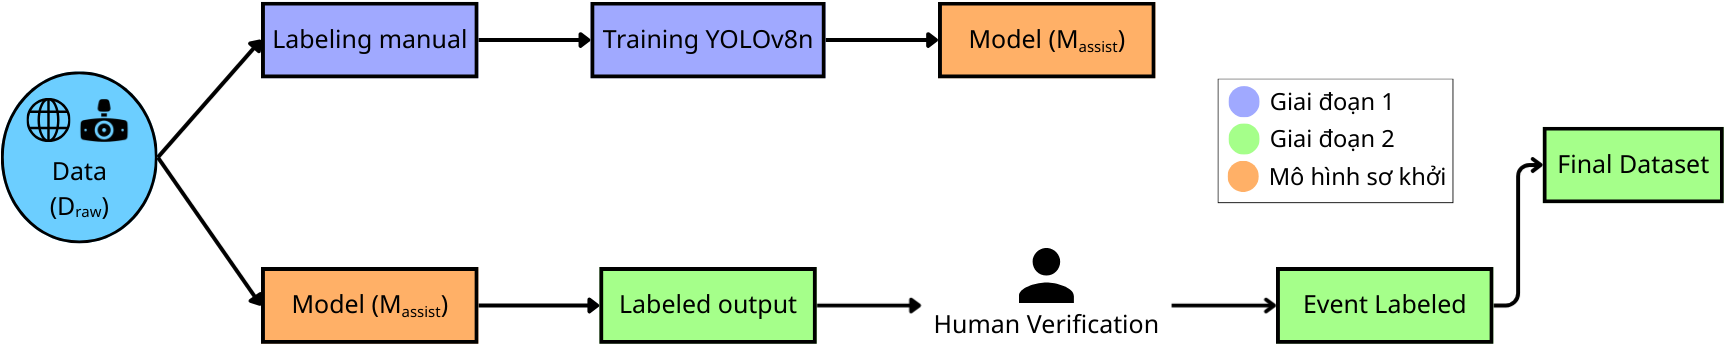
\includegraphics[width=\linewidth]{images/data_pipeline.png}
		\caption{Sơ đồ tổng quan quy trình xây dựng dữ liệu hai giai đoạn}
		\label{fig:data_pipeline}
	\end{figure}
	
	\subsubsection{Giai đoạn 1: Thiết lập Mô hình Hỗ trợ (Bootstrap Phase)}
	Mục tiêu của giai đoạn này là giải quyết bài toán Cold Start bằng cách huấn luyện một mô hình sơ khởi từ tập dữ liệu hạt giống ($D_{seed}$).
	
	\paragraph{Quy trình Tạo tập dữ liệu hạt giống ($D_{seed}$):}
	Chúng tôi trích xuất ngẫu nhiên khoảng 10-15\% tổng số lượng khung hình từ dữ liệu thô ($D_{raw}$). Các khung hình này được gán nhãn thủ công trên công cụ CVAT tuân thủ nghiêm ngặt các tiêu chuẩn sau:
	\begin{itemize}
		\item \textbf{Định nghĩa Lớp hành vi:} Xác định Bounding Box và phân loại hành vi động (\texttt{lane\_keeping}, \texttt{moving\_away}, \texttt{cut\_in}) như Hình \ref{fig:labeling}.
		\item \textbf{Định nghĩa Vùng an toàn (Heuristic Approach):} Đối với các nhãn không gian tĩnh (\texttt{Danger Zone}, \texttt{Warning Zone}), thay vì áp dụng cứng nhắc các công thức khoảng cách tiêu chuẩn phương Tây (vốn gây ra cảnh báo rác trong điều kiện giao thông xe máy dày đặc tại Việt Nam), nghiên cứu thiết lập kích thước vùng dựa trên \textit{kinh nghiệm thực tiễn}. Các đa giác được tinh chỉnh dựa trên quan sát góc nhìn thực tế của tài xế, đảm bảo phản ánh đúng không gian cần thiết cho hành vi phanh khẩn cấp trong giao thông nội đô.
	\end{itemize}
	
	\begin{figure}[!h]
		\centering
		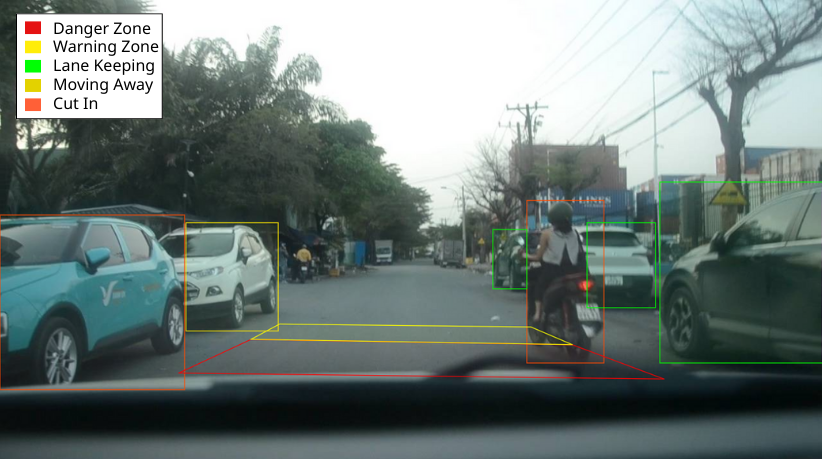
\includegraphics[width=12cm,height=5cm,keepaspectratio]{images/labeling.png}
		\caption{Minh họa gán nhãn đối tượng}
		\label{fig:labeling}
	\end{figure}
	
	\paragraph{Cấu hình Mô hình $M_{assist}$:}
	Mô hình được chọn là YOLOv8 (phiên bản nano) nhờ sự cân bằng giữa tốc độ và độ chính xác \cite{Lv2023DETRsBY}. Chiến lược Transfer Learning từ trọng số COCO được áp dụng để tăng tốc độ hội tụ. Mục tiêu của $M_{assist}$ là tối ưu hóa độ nhạy để hạn chế tối đa việc bỏ sót đối tượng (False Negative).
	
	\paragraph{Tiêu chí Chuyển tiếp (Transition Criteria):}
	Mô hình $M_{assist}$ chỉ được chấp nhận đưa vào hỗ trợ Giai đoạn 2 khi đạt ngưỡng hiệu suất: mAP@50 $\geq$ 0.9. Ngưỡng này đảm bảo chất lượng gợi ý thị giác đủ tốt để giảm tải thao tác thủ công nhưng vẫn duy trì độ tin cậy \cite{Branson2010VisualRW}.
	
	\subsubsection{Giai đoạn 2: Quy trình Gán nhãn Bán tự động (Semi-automated Labeling)}
	Sau khi đạt chuẩn, $M_{assist}$ được áp dụng cho 85-90\% dữ liệu còn lại theo quy trình:
	\begin{enumerate}
		\item \textbf{Tiền gán nhãn:} Mô hình sinh dự đoán bounding box và gán nhãn mặc định \texttt{lane\_keeping} (lớp đa số) cho toàn bộ dữ liệu.
		\item \textbf{Hiệu chỉnh:} Sử dụng CVAT để tinh chỉnh kích thước box và chỉ cần thay đổi nhãn sự kiện tại các thời điểm phát hiện hành vi bất thường (tạt đầu, rẽ), thay vì vẽ lại từ đầu.
		\item \textbf{Đóng gói:} Dữ liệu sau hiệu chỉnh được hợp nhất và kiểm tra ngẫu nhiên lần cuối.
	\end{enumerate}
	
	\subsection{Mô hình Nhận thức Hành vi}
	
	Thay vì yêu cầu mạng YOLO phải trực tiếp nhận diện một hành vi mang tính quá trình như "cắt mặt" trên một khung hình tĩnh duy nhất, đề tài xây dựng kiến trúc kết hợp: YOLO26n đóng vai trò trích xuất chuỗi đặc trưng hình học, trong khi LSTM đảm nhiệm phân loại chuỗi thời gian.
	
	\subsubsection{Mạng Trích xuất Đặc trưng Không gian (YOLO26n)}
	
	Việc lựa chọn backbone phù hợp là yếu tố then chốt để đảm bảo khả năng vận hành thời gian thực. Dựa trên phân tích so sánh chuyên sâu \cite{Hidayatullah2025YOLOv8TY}, nghiên cứu tiến hành thực nghiệm đối chiếu giữa hai biến thể:
	\begin{itemize}
		\item \textbf{YOLO26n}: Là một mô hình đầu cuối (end-to-end) thiết kế đặc biệt cho thiết bị biên. Kiến trúc này loại bỏ hoàn toàn lớp hậu xử lý NMS và tối ưu hóa thuật toán MuSGD, giúp mô hình ổn định và hội tụ nhanh hơn \cite{yolo26_ultralytics}.
		\item \textbf{YOLOv10n}: Phiên bản YOLO cải tiến từ YOLOv8, được tối ưu cho phát hiện thời gian thực với kiến trúc gọn hơn.
	\end{itemize}
	
	\begin{table}[h]
		\centering
		\caption{So sánh thông số kỹ thuật các biến thể YOLO (Phiên bản Nano) trên độ phân giải $640 \times 640$.}
		\label{tab:yolo_comparison}
		\resizebox{\linewidth}{!}{%
			\begin{tabular}{lcccc}
				\toprule
				\textbf{Model} & \textbf{mAP$^{val}_{50-95}$} & \textbf{Tham số (M)} & \textbf{FLOPs (B)} & \textbf{Năm} \\
				\midrule
				YOLO26n & \textbf{40.9} & 2.4 & \textbf{5.4} & 2026 \\
				YOLOv10n & 39.5 & \textbf{2.3} & 6.7 & 2024 \\
				\bottomrule
			\end{tabular}%
		}
		\footnotesize{\textit{*Ghi chú: Số liệu Inference đo trên T4 GPU (TensorRT FP16) theo công bố của Ultralytics.}}
	\end{table}
	
	Dựa trên số liệu Bảng \ref{tab:yolo_comparison}, YOLO26n thể hiện sự vượt trội về cả độ chính xác (40.9\% mAP) lẫn chi phí tính toán (chỉ 5.4 BFLOPs), giúp duy trì độ trễ xử lý cực thấp. Khả năng trích xuất Bounding Box chính xác và mượt mà của YOLO26n cung cấp nền tảng dữ liệu sạch, chống nhiễu tuyệt vời cho mạng LSTM ở giai đoạn sau.
	
	\begin{figure}[!h]
		\centering
		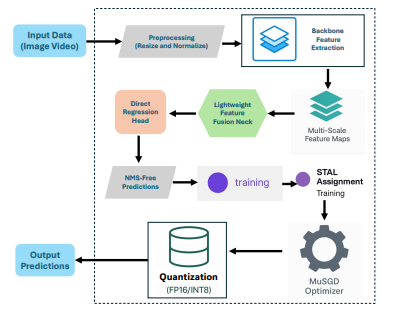
\includegraphics[width=7cm,height=7cm,keepaspectratio]{images/core_arch_yolo26.png}
		\caption{Kiến trúc YOLO26 \cite{Sapkota2025UltralyticsYE}}
		\label{fig:core_arch_yolo26}
	\end{figure}
	
	\subsubsection{Mạng Nhận thức Ý định Chuỗi Thời gian (LSTM)}
	
	Để chuyển đổi từ kết quả nhận diện vật thể sang việc hiểu hành vi, luồng dữ liệu theo dõi từ YOLO26n được đưa vào mạng LSTM để phân loại ý định.
	
	\paragraph{Cấu trúc Vector đầu vào:}
	Tại mỗi khung hình $t$, hệ thống trích xuất một vector đặc trưng không gian $V_t$ của phương tiện được theo dõi:
	\begin{equation}
		V_t = [cx_t, cy_t, w_t, h_t, conf_t]
	\end{equation}
	Trong đó, $cx, cy, w, h$ là tọa độ tâm, chiều rộng, chiều cao của Bounding Box đã được chuẩn hóa theo kích thước ảnh, và $conf$ là độ tin cậy. Việc cấp dữ liệu chuỗi $(w_t, h_t)$ liên tục cho LSTM giúp mạng tự động học được các đặc trưng vi phân bậc cao như sự biến thiên tỷ lệ khung hình ($\Delta AR$) và gia tốc ngang -- vốn là các dấu hiệu đặc trưng nhất khi xe máy nghiêng người chuẩn bị tạt đầu.
	
	\paragraph{Thiết kế Cửa sổ Thời gian:}
	Thay vì lấy các khung hình liên tiếp vốn có sự thay đổi quá nhỏ, hệ thống áp dụng kỹ thuật lấy mẫu thưa. Cụ thể, mô hình sử dụng một bộ đệm độ dài cửa sổ trạng thái $N=160$ với bước nhảy $S=3$. Do đó, để tạo ra một chuỗi gồm 10 điểm dữ liệu, hệ thống bao quát một trường nhìn thời gian khoảng 30 khung hình (tương đương $\approx 1$ giây với camera 30 FPS). Thiết kế này giúp mô hình LSTM nắm bắt được bối cảnh chuyển động đủ dài để nhận diện rõ ràng sự thay đổi quỹ đạo, vượt trội hoàn toàn so với việc đánh giá trên khung hình đơn lẻ.
	
	\subsection{Cơ chế Huấn luyện Mạng Lai}
	Quá trình huấn luyện hệ thống được chia làm hai giai đoạn độc lập để tối ưu hóa đặc thù của từng kiến trúc mạng.
	
	\paragraph{1. Huấn luyện Bộ trích xuất Không gian (YOLO26n):}
	Mô hình được huấn luyện trên cấu hình GPU Tesla T4, sử dụng bộ tối ưu hóa lai \textbf{MuSGD} kết hợp với chiến lược STAL (Spatio-Temporal Assignment Learning). Kiến trúc loại bỏ DFL (Distribution Focal Loss) và NMS giúp tối giản hóa quá trình hội tụ. Bên cạnh đó, việc sử dụng các kỹ thuật tăng cường dữ liệu từ Albumentations (CLAHE, Blur, ToGray) giúp mô hình thích nghi mạnh mẽ với điều kiện môi trường giao thông phức tạp.
	
	\paragraph{2. Huấn luyện Bộ phân loại Ý định (LSTM):}
	Sau khi mô hình YOLO đã ổn định, hệ thống tiến hành trích xuất quỹ đạo Bounding Box của tập dữ liệu huấn luyện để tạo thành các tensor chuỗi kích thước $(Batch, N, 5)$. Mạng LSTM gồm 2 lớp ẩn (Hidden size = 64, Dropout = 0.2) được huấn luyện bằng hàm mất mát CrossEntropyLoss kết hợp bộ tối ưu hóa Adam. Mạng thực hiện bài toán phân loại nhị phân (0: An toàn, 1: Có ý định cắt mặt) tại bước thời gian cuối cùng của chuỗi.
	
	\subsection{Hậu xử lý \& Logic Cảnh báo Đa tầng}
	
	Hệ thống kết hợp sức mạnh dự đoán sớm của mạng LSTM với sự chắc chắn về không gian của Luật tĩnh (Rule-based Zones) để tạo ra cơ chế Quyết định Lai (Hybrid Decision Making), đảm bảo tính an toàn tối đa.
	
	Logic cảnh báo được phân cấp dựa trên sự giao cắt giữa Bounding Box của phương tiện và đa giác ranh giới (\texttt{Danger Zone}, \texttt{Warning Zone}) kết hợp với tín hiệu ý định:
	
	\begin{itemize}
		\item \textbf{Cấp độ 1 (An toàn):} Phương tiện nằm ngoài các vùng rủi ro và mạng LSTM dự đoán ý định là 0 (Đi thẳng). Trạng thái theo dõi bình thường.
		\item \textbf{Cấp độ 2 (Theo dõi Ý định):} Mạng LSTM phát tín hiệu 1 (Có ý định tạt đầu), nhưng phương tiện vẫn còn ở xa, chưa chạm vào bất kỳ Zone cảnh báo nào. Hệ thống đánh dấu phương tiện nhưng chưa phát âm thanh.
		\item \textbf{Cấp độ 3 (Cảnh báo):} Phương tiện đã giao cắt vào \texttt{Warning Zone} VÀ đồng thời LSTM phát tín hiệu 1. Tại đây, rủi ro cắt mặt đã rất rõ ràng, hệ thống kích hoạt cảnh báo mức độ trung bình (Cam).
		\item \textbf{Cấp độ 4 (Khẩn cấp - Danger Override):} Phương tiện tiến sâu và giao cắt với \texttt{Danger Zone}. Hệ thống bỏ qua mọi dự đoán của AI (Override) và kích hoạt cảnh báo Đỏ ngay lập tức do rủi ro va chạm vật lý là tất yếu.
	\end{itemize}
	
	Sự kết hợp logic lai này giúp hệ thống vừa có năng lực "cảnh báo sớm" (nhờ LSTM), vừa đảm bảo nguyên tắc "không bao giờ bỏ lọt" (nhờ Rule-based Zones) trong các tình huống khẩn cấp thực tế.